\chapter{Solución de ecuaciones lineales de dimensiones no pequeñas}\label{chapter:solve-non-smal-lineal-eq}

En el capítulo anterior, se presentó la discretización Lineal Local~(\ref{ODE-LLA-4}) de EDO, así como su implementación~(\ref{LL-scheme}) para PVI de dimensiones pequeñas. Sin embargo, para PVI de medianas y grandes dimensiones, la aproximación de Padé~(\ref{P-MA-2}) utilizada en (\ref{LL-scheme}) para aproximar (\ref{ODE-LLA-4}) no es computacionalmente eficiente y necesita ser reemplazada por otra aproximación basada en subespacios de Krylov o alguna técnica proyectiva similar. Nótese que, para la ecuación lineal
\begin{equation*}
	\frac{dx(t)}{dt}=Ax(t)\;,\;\; x(t_0)=x_0\in\mathbb{R}^{d},\;\;\; A\in\mathbb{R}^{d\times d},\;\;t\geq t_0\in\mathbb{R} \,,
\end{equation*}
además de la solución en forma integral, la solución también puede ser escrita de las siguientes formas
\begin{eqnarray}
	x(t) & = & \me{(t-t_0)A}x_0 \label{eqaux:lineal-solution-ex} \\
	x(t) & = & x_0 + \lmatrix\me{(t-t_0)M}\rvector \label{eqaux:lineal-solution-xex} \\
	x(t) & = & x_0 + (t-t_0)\varphi_1((t-t_0)A)Ax_0 \label{eqaux:lineal-solution-xphix}
\end{eqnarray}
donde $\varphi_1$ está definida en (\ref{phi-definition}) y
\begin{equation*}
	\lmatrix=\left[ \begin{array}{ll} I_{d} & 0_{d\times 1}\end{array} \right] \;,\;\;
	\rvector^{\intercal }=\left[ \begin{array}{ll} 0_{1\times d} & 1\end{array}\right] \;,\;\;
	M=\left[
	\begin{array}{cc}
	A & Ax_0 \\
	0 & 0
	\end{array}
	\right]\;.
\end{equation*}
Cada una de estas formas de la solución puede ser aproximada utilizando subespacios Krylov. Apoyandose en el resultado del Teorema \ref{exp-bound}, en los trabajos~\cite{hochbruck1998exponential,jimenez2012convergence} se utilizaron aproximaciones de Krylov para las soluciones de las forma~(\ref{eqaux:lineal-solution-ex}) y~(\ref{eqaux:lineal-solution-xex}). Dichas aproximaciones son de orden $\mf$, donde $\mf$ es la dimensión del subespacio utilizado. En cambio para la solución de la forma~(\ref{eqaux:lineal-solution-xphix}) se han utilizado aproximaciones de orden  $\mf+1$ derivadas del truncamiento de la serie (\ref{PHI-EXPANSION})~\cite{sidje1998expokit,niesen2012algorithm}. En este capítulo, empleando nuevamante la serie (\ref{PHI-EXPANSION}), se introducirán aproximaciones Krylov-Padé de un orden mayor para la acción de $\varphi_1$ sobre un vector, así como una variante de dicha aproximación que no evalúa la matriz Jacobiana. También se derivarán cotas para las aproximaciones propuestas y se propondrá una estrategia para la selección de la dimensión de los subespacios de Krylov. Los resultados de este capítulo están basados en \cite{naranjo2023computing,naranjo2023RT,naranjo2021locally,naranjo2023jacobian}.

\section{Aproximaciones Krylov-Padé a la acción del operador phi}\label{section:krylov-pade-approx}

Como se comentó en la Sección \ref{section:phi-times-vector}, la acción del operador $\varphi_1$ definida como el producto de la función $\varphi_1$ por vector tiene un papel fundamental en las discretizaciones Lineales Locales de la solución de ecuaciones lineales autónomas, por lo que se hace indispensable evaluar dicha operación de forma rápida y precisa. Con ese propósito, el truncamiento de la serie~(\ref{PHI-EXPANSION}) es útil. Típicamente~\cite{niesen2012algorithm,sidje1998expokit,tokman2006efficient}, el primer término de dicha serie es tomado como aproximación y el segundo término es utilizado como medida del error. Sin embargo, en este trabajo, similar a~\cite{Saad92} se tomarán los dos primeros términos
\importantdefinition{$K_\mf(\tau,A,b)$ aproximación de Krylov para $\tau\varphi_1(\tau A)b$}
 \begin{equation}\label{exact-two-terms-km}
    K_\mf(\tau,A,b) = \norme{b}\tau V_\mf\varphi_1(\tau H_\mf)e_1 + \norme{b}\tau^2\hf_{\mf+1,\mf}e^\intercal_\mf\varphi_2(\tau H_\mf)e_1v_{\mf+1}
 \end{equation}
de la serie (\ref{PHI-EXPANSION}) para aproximar $\tau\varphi_1(\tau A)b$ y el tercer término como medida del error.

Al aplicar conjuntamente el Algoritmo de Arnoldi \ref{alg:Arnoldi}, la propiedad de invarianza ante escalado de la base ortonormal del subespacio de Krylov y el Teorema \ref{theorem:exp-phi} podemos evaluar la acción de las $\varphi_j$ en (\ref{exact-two-terms-km}) calculando una sola exponencial matricial. En efecto, con la matriz de Hessenberg $H^*_\mf$ resultante de aplicar el Algoritmo \ref{alg:Arnoldi} para $\mathcal{K}_\mf(\tau A,b)$ se obtiene la matriz de Hessenberg $H_\mf=H^*_\mf/\tau$ correspondiente a $\mathcal{K}_\mf(A,b)$ y, de ésta forma, se puede calcular la exponencial de la matriz particionada
\begin{equation}
    \overline{H} = \left[\begin{array}{cccc}
    H_\mf & e_1 & 0_{\mf\times 1} & 0_{\mf\times 1}\\
    0_{1\times\mf} & 0 & 1 & 0\\
    0_{1\times\mf} & 0 & 0 & 1\\
    0_{1\times\mf} & 0 & 0 & 0
    \end{array}\right] \label{hhat_hessenberg_matrix}
    \end{equation}
para obtener la identidad
\begin{equation}
    \me{\tau\overline{H}} = \left[\begin{array}{cccc}
    \me{\tau H_m} & \tau\varphi_1(\tau H_m)e_1 & \tau^{2}\varphi_2(\tau H_m)e_1 &
    \tau^{3}\varphi_3(\tau H_m)e_1 \\
    \bluemark{0_{1\times\mf}} & 1 & \tau & \frac{\tau^{2}}{2}\\
    \bluemark{0_{1\times\mf}} & 0 & 1 & \tau \\
    \bluemark{0_{1\times\mf}} & 0 & 0 & 1 \\
    \end{array}\right] \,. \label{phi_hhat_exponential}
\end{equation}
del Teorema \ref{theorem:exp-phi}.

Al aplicar (\ref{phi_hhat_exponential}) en (\ref{exact-two-terms-km}) se obtiene
\begin{equation*}
    K_\mf(\tau,A,b) = \norme{b}V_\mf [E_\tau]_{12} + \norme{b}\hf_{\mf+1,\mf}e^\intercal_\mf[E_\tau]_{13}v_{\mf+1}, 
 \end{equation*}
 donde $E_\tau = \me{\tau \overline{H} }$ y $[E_\tau]_{ij}$ denota las particiones de la matriz $E_\tau$ análogas a las particiones de la matriz (\ref{hhat_hessenberg_matrix}). Como, en general, la exponencial matricial $E_\tau$ no se puede calcular de forma exacta, se utiliza la aproximación
\begin{equation*}
    \widetilde{E}_{\tau} = F_k^{\pf,\qf}\left(\tau\overline{H}\right),
\end{equation*}
donde $F_k^{\pf,\qf}$ denota la aproximación de Padé-($\pf,\qf$) con escalamiento y potenciación $k$ definida en~(\ref{P-MA-2}). Con esta nueva aproximación, se obtiene la expresión 
\importantdefinition{$K_{\mf,k}^{\pf,\qf}(\tau,A,b)$ aproximación de Krylov-Padé para $\tau\varphi_1(\tau A)b$}
\begin{equation} \label{eq:kp_aprox}
    K_{\mf,k}^{\pf,\qf}(\tau,A,b) = \norme{b}V_\mf [\widetilde{E}_\tau]_{12} + \norme{b}\hf_{\mf+1,\mf}e^\intercal_\mf[\widetilde{E}_\tau]_{13}v_{\mf+1}
 \end{equation}
 que define a la aproximación de Krylov-Padé para $\tau\varphi_1(\tau A)b$.

 \subsection{Cotas para las aproximaciones}
 En esta sección se enunciará un teorema para acotar el error de la aproximación Krylov-Padé (\ref{eq:kp_aprox}) en función de $\tau$, la dimensión del subespacio de Krylov $\mf$, los órdenes de Padé $\pf$ y $\qf$, \redmark{y la norma $||A||_2$}. Para poder demostrar dicho teorema se necesitan dos lemas adicionales. El primer lema extiende los resultados del Teorema 4.7 en~\cite{Saad92} para aproximaciones de $\varphi_0(A)b$ mediante subespacios de Krylov a $\tau \varphi_1(\tau A)b$. El segundo lema establece una cota para la matriz $\overline{H}$. 

 \begin{lemma}\cite{naranjo2021locally}\label{lemma:CORRECTED-ERROR}
	Sea $A\in\mathbb{C}^{d\times d}$ una matriz, $b\in\mathbb{C}^{d}$ un vector, $\tau$ un número positivo, y 
	\begin{equation}
		{K_{\mf}\left(\tau,A , b \right) = \tau ||b||_2 V_\mf \varphi_1(\tau H_\mf)e_1}+\tau^2 ||b||_2 \hf_{\mf+1,\mf}e_\mf^\intercal\varphi_2\left(\tau H_\mf\right) e_1 v_{\mf+1} \label{eq:km-exact-222}
	\end{equation}
	 la aproximación a $\tau \varphi_1(\tau A)b$ tomando los dos primeros términos de la serie (\ref{PHI-EXPANSION}). Entonces,
	\begin{gather*}
	\left\lvert\left\lvert \tau\varphi_1(\tau A)b - K_{\mf}\left(\tau,A , b \right) \right\rvert\right\rvert_2%\nonumber\\
	\leq \frac{2\vert\lvert b \rvert\rvert_2\tau^{\mf+2}\rho^{\mf+1}\me{\tau \rho}}{(\mf+2)!},
	\end{gather*}
	donde $\rho=\nnorm{\nnorm{A}}_2$.
\end{lemma}
\textbf{Demostración.}
Siguiendo la definición (\ref{phi-definition}), $\tau \varphi_1(\tau A)b$ puede ser reescrito como
\begin{eqnarray*}
	\tau \varphi_1(\tau A)b &=& \tau b+\tau^{2}A\varphi_{2}(\tau A)b \\
	&=& \tau b+\tau^{2}A \,\ (\,\ \nnorm{\nnorm{b}}_2V_\mf\varphi_{2}(\tau H_\mf)e_1 +s_\mf(\tau A) \,\ ), %\label{eq:tauaphi1tauab}
\end{eqnarray*}
donde \[ s_\mf (\tau A)= \varphi_{2}(\tau A)b -\nnorm{\nnorm{b}}_2V_\mf\varphi_{2}(\tau H_\mf)e_1 .\]
Utilizando la rescritura de $\varphi_1$, y las identidades $AV_\mf=V_\mf H_\mf + \hf_{\mf+1,\mf}v_{\mf+1}e^\intercal_\mf$ y  $\nnorm{\nnorm{b}}_2V_\mf e_1=b$ se obtiene
\begin{equation}
\tau\varphi_1(\tau A)b = \tau\nnorm{\nnorm{b}}_2V_\mf\varphi_1(\tau H_\mf)e_1 + \tau^{2}\nnorm{\nnorm{b}}_2\hf_{\mf+1,\mf}e^\intercal_\mf\varphi_{2}(\tau H_\mf)e_1v_{\mf+1}+\tau^{2}As_\mf (\tau A), %\label{eq:tauaphi1tauabapprox}
\end{equation}
y se tiene que
\begin{equation}
\tau\varphi_1(\tau A)b - K_{\mf}\left(\tau,A , b \right) = \tau^{2}As_\mf(\tau A), \label{eq:phidiffasm}
\end{equation}
donde $K_{\mf}\left(\tau,A , b \right)$ definida en (\ref{eq:km-exact-222}) es una aproximación de $\tau \varphi_1(\tau A)b$.

Utilizando el Lema 4.1 en \cite{Saad92} se tiene
\begin{equation}
s_\mf(\tau A)=\nnorm{\nnorm{b}}_2 ( r_\mf(\tau A)v_1-V_\mf r_\mf(\tau H_\mf)e_1) ,\label{eq:smeq}
\end{equation}
donde $r_\mf(z) = \varphi_{2}(z)-p_{2,\mf-1}(z)$, y $p_{2,\mf-1}$ es un polinomio de grado $\mf-1$. En virtud de la arbitrariedad para \bluemark{$p_{2,\mf-1}$}, definimos
\begin{equation*}
p_{2,\mf-1}(z)\equiv \frac{p_{1,\mf}(z)-1}{z},
\end{equation*}
donde $p_{1,\mf}$ es la expansión de Taylor de $\varphi_1$ hasta el orden  $\mf$
definida por
\[ p_{1,\mf}(z)= \frac{p_{0,\mf+1}(z)-1}{z}, \]
siendo $p_{0,\mf+1}(z)$ la expansión de Taylor de $\me{z}$ hasta el orden $\mf+1$ dada por
\[ p_{0,m+1}(z)=\sum\limits^{\mf+1}_{j=0}\frac{z^j}{j!}. \]

Con estos polinomios y (\ref{phi-definition}) se tiene
\begin{equation*}
r_\mf(z) = \frac{\varphi_1(z)-1}{z}-\frac{p_{1,\mf}(z)-1}{z}=\frac{\me{z}-1}{z^2}-\frac{p_{0,m+1}(z)-1}{z^2}
=\frac{\me{z}-p_{0,m+1}(z)}{z^2}.
\end{equation*}

El Lema 4.2 en \cite{Saad92} enuncia que
\[ \nnorm{\me{z}-p_{0,m+1}(z)} \leq \frac{z^{\mf+2}\me{z}}{(\mf+2)!}\;\;, \]
de donde se obtiene
\begin{equation}
\nnorm{\nnorm{r_\mf(\tau A)v_1}}_2\leq \frac{\rho^{\mf}\me{\rho}}{(\mf+2)!}\;\;\;\;\; y \;\;\;\;\; \nnorm{\nnorm{r_\mf(\tau H_\mf)v_1}}_2\leq \frac{\widehat{\rho}^{\mf}\me{\widehat{\rho}}}{(\mf+2)!}, \label{polinom}
\end{equation}
con $\rho=\nnorm{\nnorm{\tau A}}_2 $ y  $\widehat{\rho}=\nnorm{\nnorm{\tau H_\mf}}_2$. Teniendo en cuenta que $\nnorm{\nnorm{H_\mf}}_2\leq\nnorm{\nnorm{A}}_2$, de (\ref{eq:smeq}) y (\ref{polinom}) se obtiene
\begin{equation*}
\nnorm{\nnorm{\tau As_\mf(\tau A)}}_2  \leq \frac{2 \nnorm{\nnorm{b}}_2\rho^{\mf+1}\me{\rho}}{(\mf+2)!}.
\end{equation*}
Finalmente, de la desigualdad anterior y (\ref{eq:phidiffasm}) se obtiene
\begin{equation*}
\nnorm{\nnorm{\tau\varphi_1(\tau A)b - K_{\mf}\left(\tau,A , b \right)}}_2  \leq
\frac{2 \nnorm{\nnorm{b}}_2\tau^{\mf+2}\nnorm{\nnorm{A}}_2^{\mf+1}\me{\tau \nnorm{\nnorm{A}}_2}}{(\mf+2)!},
\end{equation*}
lo cual completa la prueba. $\Box$

\begin{lemma}\cite{naranjo2021locally}\label{H-bound}
	Sea $\overline{H}$ la matriz definida en~(\ref{hhat_hessenberg_matrix}) y $H_\mf=V^\intercal_\mf AV_\mf$ la matriz de Hessenberg asociada al subespacio de Krylov $\mathcal{K}_\mf(A,b)$ con base ortonormal $V_m$. Entonces
	\[ \lVert\overline{H}\rVert_2 \leq 1 +  \lVert A\rVert_2. \]
\end{lemma}
\textbf{Demostración.}
De (\ref{hhat_hessenberg_matrix}) se tiene
\begin{eqnarray*}
	\overline{H}&=&\lmatrix H_\mf \lmatrix^\intercal + B\,,
\end{eqnarray*}
donde $ \lmatrix^\intercal=[I_\mf \;\; 0_{\mf\times 3}] $ y
\[B=\left[\begin{array}{ccc}
0_{\mf\times\mf} & e_1 & 0_{\mf \times 2}\\
0_{2\times\mf} & 0_{2 \times 1} & I_2\\
0_{1\times\mf} & 0 & 0_{1\times 2}
\end{array}\right].\]
Como $\lVert B\rVert_2 = \lVert \lmatrix \rVert_2 = 1$, y $\lVert H_m\rVert_2 \le \lVert A \rVert_2$, se obtiene que
\begin{eqnarray*}
	\lVert\overline{H}\rVert_2 &\leq& \lVert \lmatrix \rVert_2 \lVert H_\mf \rVert_2 \lVert \lmatrix^\intercal \rVert_2 + \lVert B \rVert_2\\
	&\leq& 1 + \lVert A\rVert_2
\end{eqnarray*}
$\Box$\\ \\


\begin{theorem}\cite{naranjo2021locally}\label{theorem:Krylov-bound}
	Sea
	\begin{equation} \label{eq:gen_kp_aprox}
	K_{\mf,k}^{\pf,\qf}\left(\tau, A , b \right)=\nnorm{\nnorm{b}}_2 V_{\mf}\;[\widetilde{E}_{\tau}]_{12} + \nnorm{\nnorm{b}}_2 \hf_{\mf+1,\mf}e_\mf^\intercal\;[\widetilde{E}_{\tau}]_{13} v_{\mf+1}
	\end{equation}
	la aproximación $(\mf , \pf ,\qf , k)$-Krylov-Padé de $\tau \varphi_1(\tau A)b$, donde las matrices $V_{\mf}\in\mathbb{R}^{d\times \mf}$ y $H_{\mf}\in\mathbb{R}^{{\mf} \times {\mf}}$, el vector $v_{\mf+1}$, y el número $\hf_{\mf+1,\mf}$ son obtenidos del Algoritmo de Arnoldi para el $\mf$-ésimo subespacio de Krylov $\mathcal{K}_\mf(A,b)$;  $\widetilde{E}_{\tau}=F_k^{\pf,\qf}\left(\tau\overline{H}\right)$ es la aproximación $(\pf,\qf)$-Padé con escalamiento $k$ para la exponencial matricial (\ref{phi_hhat_exponential}), y $e_m$ el $m$-ésimo vector canónico de $\mathbb{R}^\mf$.
	Entonces,
	\begin{equation}
	\left\lvert\left\lvert  \tau \varphi_1(\tau A)b -
	K_{\mf,k}^{\pf,\qf}\left( \tau, A , b \right)\right\rvert\right\rvert_2%\nonumber\\
	\leq C_{\mf,k}^{\pf,\qf}\left(\lvert\lvert A \rvert\rvert_2\right) \;
	\nnorm{\nnorm{b}}_2 \; \tau^{\mathrm{min}\left\{ \mf+2,\pf+\qf+1 \right\}}
	\end{equation}
	donde $C_{\mf,k}^{\pf,\qf}(\varLambda)= \frac{2 \varLambda^{m+1} \me{\varLambda}}{(\mf+2)!}+
	\alpha (1+\hf_{\mf+1,\mf}) (1+\varLambda^{p+q+1}) 2^{-k(\pf+\qf)+3}\me{(1+\alpha(\frac{1}{2})^{\pf+\qf-3})(1+\varLambda)} $,
	con $\alpha=\frac{\pf!\qf!}{(\pf+\qf)!(\pf+\qf+1)!}$ y $\tau \in [0,1]$.
\end{theorem}
\textbf{Demostración.} Por desigualdad triangular
\begin{eqnarray} \label{importatdeq}
\left\lvert\left\lvert  \tau \varphi_1(\tau A)b -
K_{\mf,k}^{\pf,\qf}\left( \tau , A , b \right)\right\rvert\right\rvert_2
& \leq & \left\lvert\left\lvert \tau \phi_1(\tau A)b -  K_{\mf}\left( \tau , A , b \right) \right\rvert\right\rvert_2 \\
& & + \left\lvert\left\lvert  K_{\mf}\left( \tau , A , b \right) -
K_{\mf,k}^{\pf,\qf}\left( \tau, A , b \right)\right\rvert\right\rvert_2, \nonumber
\end{eqnarray}
donde
\begin{equation*}
K_{\mf}\left(\tau,A , b \right)=\nnorm{\nnorm{b}}_2 \tau V_{\mf}\varphi_1\left( \tau H_{\mf} \right) e_1 + \nnorm{\nnorm{b}}_2 \tau^{2}\hf_{\mf+1,\mf}e_\mf^\intercal\varphi_2\left(\tau H_\mf\right) e_1 v_{\mf+1}
\end{equation*}
es la aproximación de Krylov de $\tau \varphi_1(\tau A)b$ definida en~(\ref{exact-two-terms-km}), y
\begin{equation*}
K_{\mf,k}^{\pf,\qf}\left(\tau, A , b \right)=\nnorm{\nnorm{b}}_2 V_{\mf}\;[\widetilde{E}_{\tau}]_{12} + \nnorm{\nnorm{b}}_2 \hf_{\mf+1,\mf}e_\mf^\intercal\;[\widetilde{E}_{\tau}]_{13} v_{\mf+1}
\end{equation*}
la aproximación Krylov-Padé de $\tau \varphi_1(\tau A)b$ definida en~(\ref{eq:kp_aprox}).

De (\ref{phi_hhat_exponential}) se tiene que
$\tau^j \varphi_j\left( \tau H_{\mf} \right) e_1 = \lmatrix \me{\tau \overline{H}} \rvector_j$
y
$[\widetilde{E}_{\tau}]_{1,j+1} = \lmatrix F_k^{\pf,\qf}(\tau \overline{H}) \rvector_j$,
con $j=1,2$, donde $F_k^{\pf,\qf}(\tau \overline{H})$ es la aproximación $(\pf,\qf)$-Padé de $\me{\tau \overline{H}}$ con estrategia escalamiento y potenciación,
$ \lmatrix=[I_\mf \;\; 0_{\mf\times 3}] $, $\rvector_1=[0_{1\times \mf}\;\; 1 \;\;0 \;\;0]^\intercal$ y $\rvector_2=[0_{1\times \mf}\;\; 0 \;\;1 \;\;0]^\intercal$. De la desigualdad triangular
\begin{equation}\label{proffktheouneq}
%\begin{array}{ccc}
\left\lvert\left\lvert   K_{\mf}\left( \tau , A , b \right) -
K_{\mf,k}^{\pf,\qf}\left( \tau, A , b \right)\right\rvert\right\rvert_2
\leq \left\lvert\left\lvert T_1 -
\widetilde{T}_1\right\rvert\right\rvert_2 \\
+\left\lvert\left\lvert T_2 - \widetilde{T}_2
\right\rvert\right\rvert_2,
%\end{array}
\end{equation}
donde
\begin{eqnarray*}
	T_1&=&\nnorm{\nnorm{b}}_2 V_{\mf} \lmatrix \me{\tau \overline{H}} \rvector_1\\
	\widetilde{T}_1&=&\nnorm{\nnorm{b}}_2 V_{\mf} \lmatrix F_k^{\pf,\qf}(\tau \overline{H}) \rvector_1\\
	T_2&=&\nnorm{\nnorm{b}}_2 \hf_{\mf+1,\mf}e_\mf^\intercal\;\lmatrix \me{\tau \overline{H}} \rvector_2 v_{\mf+1}\\
	\widetilde{T}_2&=&\nnorm{\nnorm{b}}_2 \hf_{\mf+1,\mf}e_\mf^\intercal\;\lmatrix F_k^{\pf,\qf}(\tau \overline{H}) \rvector_2 v_{\mf+1}.
\end{eqnarray*}

Del Lema 4.1 en \cite{jimenez2012convergence} y el Lema~\ref{H-bound}, se tiene que
\begin{eqnarray}
\left\lvert\left\lvert T_1 - \widetilde{T}_1\right\rvert\right\rvert_2
&\leq& \nnorm{\nnorm{b}}_2 \left\lvert\left\lvert  V_{\mf} \right\rvert\right\rvert_2 \left\lvert\left\lvert  \lmatrix \right\rvert\right\rvert_2 \left\lvert\left\lvert \me{\tau  \overline{H}}-F_k^{\pf,\qf}(\tau \overline{H}) \right\rvert\right\rvert_2
\left\lvert\left\lvert  \rvector_1 \right\rvert\right\rvert_2 \nonumber\\
&\leq& \nnorm{\nnorm{b}}_2 \;  c_{\pf,\qf}(k,\lvert\lvert\tau\overline{H}\rvert\rvert_2) \;
\lvert\lvert\tau \overline{H}\rvert\rvert_2^{\pf+\qf+1}\nonumber\\
&\leq& \nnorm{\nnorm{b}}_2 \; c_{\pf,\qf}(k,\tau (1+\lvert\lvert A \rvert\rvert_2))
\; (1 + \lvert\lvert A \rvert\rvert_2^{\pf+\qf+1}) \; \tau^{\pf+\qf+1}
\label{err1}
\end{eqnarray}
y
\begin{eqnarray}
\left\lvert\left\lvert T_2 - \widetilde{T}_2 \right\rvert\right\rvert_2
&\leq& \nnorm{\nnorm{b}}_2 \lvert \hf_{\mf+1,\mf}\rvert \left\lvert\left\lvert  e_\mf^\intercal \right\rvert\right\rvert_2 \left\lvert\left\lvert  \lmatrix \right\rvert\right\rvert_2 \left\lvert\left\lvert \me{\tau \overline{H}}-
F_k^{\pf,\qf}(\tau \overline{H}) \right\rvert\right\rvert_2  \left\lvert\left\lvert  \rvector_2 \right\rvert\right\rvert_2 \left\lvert\left\lvert v_{\mf+1}\right\rvert\right\rvert_2 \nonumber\\
&\leq&\nnorm{\nnorm{b}}_2 \lvert \hf_{\mf+1,\mf}\rvert \; c_{\pf,\qf}
(k,\lvert\lvert\tau \overline{H}\rvert\rvert_2) \;
\lvert\lvert\tau \overline{H}\rvert\rvert_2^{\pf+\qf+1}\nonumber\\
&\leq& \nnorm{\nnorm{b}}_2 \lvert \hf_{\mf+1,\mf}\rvert \; c_{\pf,\qf}(k,\tau (1+\lvert\lvert A \rvert\rvert_2))
\; (1 + \lvert\lvert A \rvert\rvert_2^{\pf+\qf+1}) \; \tau^{\pf+\qf+1}\label{err2},
\end{eqnarray}
donde $c_{\pf,\qf}(k,\vartheta )=\alpha
2^{-k(\pf+\qf)+3}\me{(1+\alpha(\frac{1}{2})^{\pf+\qf-3})\vartheta }$ y $%
\alpha =\frac{\pf!\qf!}{(\pf+\qf)!(\pf+\qf+1)!}$. Sustituyendo (\ref{err1}) y (\ref{err2}) en (\ref{proffktheouneq}), se obtiene que
%\begin{eqnarray}
\begin{equation}
\left\lvert\left\lvert   K_{\mf}\left( \tau , A , b \right) -
K_{\mf,k}^{\pf,\qf}\left( \tau, A , b \right) \right\rvert\right\rvert_2
\leq \nnorm{\nnorm{b}}_2 (1+\lvert\hf_{\mf+1,\mf}\rvert) \; c_{\pf,\qf}(k,\tau (1+\lvert\lvert A \rvert\rvert_2))
\; (1 + \lvert\lvert A \rvert\rvert_2^{\pf+\qf+1}) \; \tau^{\pf+\qf+1}. \label{errp1}
\end{equation}
%\end{eqnarray}

Finalmente, de las desigualdades~(\ref{importatdeq}) y (\ref{errp1}), el Lema \ref{lemma:CORRECTED-ERROR}, y la condición $\tau \in [0,1]$ se obtiene
\begin{eqnarray*}
	\left\lvert\left\lvert  \tau \varphi_1(\tau A)b-  K_{\mf,k}^{\pf,\qf}\left( \tau,  A , b \right)\right\rvert\right\rvert_2
	&\leq& \frac{2 \nnorm{\nnorm{b}}_2 \tau^{\mf+2}  \vert\lvert A\rvert\rvert^{\mf+1}_2
		\me{\tau \lvert\lvert A\rvert\rvert_2}}{(\mf+2)!}\\
	&+&
	\nnorm{\nnorm{b}}_2 (1+\lvert\hf_{\mf+1,\mf}\rvert) \; c_{\pf,\qf}(k,\tau (1+\lvert\lvert A \rvert\rvert_2))
	\; (1 + \lvert\lvert A \rvert\rvert_2^{\pf+\qf+1}) \; \tau^{\pf+\qf+1}\\
	& \leq & \nnorm{\nnorm{b}}_2 C_{\mf,k}^{\pf,\qf}\left(\lvert\lvert A \rvert\rvert_2\right)\tau^{\mathrm{min}\left\{ \mf+2,\pf+\qf+1 \right\}},
\end{eqnarray*}
lo cual concluye la prueba.
$\Box$

Obsérvese que la aproximación (\ref{eq:kp_aprox}) depende de valores no especificados para la dimensión de Krylov $\mf$ y el orden de Padé ($\pf,\qf$). Más adelante, en la Sección \ref{section:approx-non-auto}, el resultado del Teorema \ref{theorem:Krylov-bound} recién demostrado será utilizado para estimar adaptativamante esos parámetros. Adicionalmente, dicho teorema es fundamental para establecer el orden de convergencia de los integradores numéricos propuestos en el Capítulo \ref{chapter:lldp}, análisis que no ha sido realizado con anterioridad por otros autores para establecer el orden de convergencia de los integradores exponenciales con aproximaciones de Krylov.

\section{Aproximaciones Krylov-Padé libre de Jacobiano a la acción del operador phi} \label{section:fj-krylov-pade-approx}
En general para PVI de grandes dimensiones la evaluación de la matriz Jacobiana $f_x$ del campo vectorial $f$ no siempre es posible, ya sea por no ser eficiente en términos de memoria u operaciones flotantes o por tener una expresión matemática difícil derivar explícitamente. En estos casos, las aproximaciones libres de Jacobiano para el producto de matrix Jacobiana por vector son necesarias~\cite{al2009complex,knoll2004jacobian}. Por construcción, la discretización Lineal Local~(\ref{ODE-LLA-4}) contiene productos de la matriz Jacobiana por vector $f_x(y)b$ que pueden ser aproximados por diferencias finitas de orden 1 \redmark{o} 2. A modo ilustrativo se tomará la diferencia finita hacia adelante
\begin{equation*}
	\frac{F(u+\delta b)-F(u)}{\delta} =  \left(\begin{array}{c}
		\frac{F_1(u_1+\delta b_1,u_2+\delta b_2)-F_1(u_1,u_2)}{\delta}\\
		\frac{F_2(u_1+\delta b_1,u_2+\delta b_2)-F_2(u_1,u_2)}{\delta}\\
	\end{array}\right)
\end{equation*}
de la función vectorial suave 2-dimensional $F(u_1,u_2)=[F_1(u_1,u_2),\,F_2(u_1,u_2)]^{\intercal}$ para aproximar el producto de la matriz Jacobiana por vector \begin{equation*}
	J(u)b = \left[\begin{array}{c}
		b_1\frac{\partial F_1(u_1,u_2)}{\partial u_1} + b_2\frac{\partial F_1(u_1,u_2)}{\partial u_2}\\
		b_1\frac{\partial F_2(u_1,u_2)}{\partial u_1} + b_2\frac{\partial F_2(u_1,u_2)}{\partial u_2}\\
	\end{array}\right],
\end{equation*}
donde $J(u)$ es la matriz Jacobiana de $F$ y $b=[b_1,b_2]^{\intercal}$ es un vector 2-dimensional. Aproximando $F(u+\delta b)$ con la expansión en serie de Taylor de primer orden en $u$, se tiene
\begin{equation*}
	\frac{F(u+\delta b)-F(u)}{\delta} =  \left(\begin{array}{c}
		\frac{F_1(u_1,u_2) + \delta b_1 \frac{\partial F_1}{\partial u_1} + \delta b_2 \frac{\partial F_1}{\partial u_2} -F_1(u_1,u_2)}{\delta}\\
		\frac{F_2(u_1,u_2) + \delta b_1 \frac{\partial F_2}{\partial u_1} + \delta b_2 \frac{\partial F_2}{\partial u_2} -F_2(u_1,u_2)}{\delta}\\
	\end{array}\right)  + O(\delta\nnnorm{b}_2^2),
\end{equation*}
y por tanto
\begin{equation*}
	\frac{F(u+\delta b)-F(u)}{\delta} =  J(u)b + O(\delta\nnnorm{b}_2^2).
\end{equation*}

En lo que resta del documento se asumirá que, si $f$ es $(\eta+1)$  continuamente diferenciable, existe una función $(\eta+1)$ continuamente diferenciable $g: \mathbb{R}^{d}\times \mathbb{R}^{d} \times \mathbb{R}_+ \to \mathbb{R}^{d}$ que aproxima al producto $f_x(y)b$ con orden $\eta$ para la cual la cota
\begin{equation} \label{eq:g_bound}
	\nnnorm{g(y,b;\delta)-f_x(y)b} \leq \mathfrak{L}\nnnorm{b}_2^{\eta+1}\delta^{\eta}
\end{equation}
se cumple, donde $f_x(y)$ es la matriz Jacobiana del campo vectorial $f$ en el punto $y$; $y,b$ son vectores $d$-dimensionales y $\mathfrak{L}$ es una constante positiva que depende solamente de la norma de las derivadas de $f_x$.

Al utilizar el Algoritmo de Arnoldi~\ref{alg:Arnoldi}, la aproximación $K_{\mf,k}^{\pf,\qf}(\tau,A,b)$ definida en~(\ref{eq:kp_aprox}) con $A=f_x(y)$ requiere de la evaluación explícita de la matriz Jacobian $f_x(y)$ para calcular su producto con diferentes vectores. Al aproximar los mencionados productos de matriz Jacobiana por vector mediante una función $g$ definida como en (\ref{eq:g_bound}) se obtine el Algoritmo de Arnoldi libre de Jacobiano~\ref{alg:iArnoldi} propuesto en \cite{brown1987local} para el subspacio de Krylov de la siguiente definición. 
\importantdefinition{$\mf$-ésimo subespacio de Krylov libre de Jacobiano}
\begin{definition}
	\cite{brown1987local} Para $\mf\geq 1$, el $\mf$-ésimo subespacio de Krylov libre de Jacobiano de la función matricial $f_x(y)\in\mathbb{R}^{N\times N}$
	y vectores $y,b\in\mathbb{R}^{N}$ se define como
	\[ \widehat{\mathcal{K}}_\mf(\tau f_x(y),b;\delta)=\mathrm{span} \left\{ b,\widehat{q}_1,\ldots,\widehat{q}_{\mf-1} \right\}. \]
	para todo $\tau, \delta > 0$, con $\widehat{q}_1=g(y,b;\delta)$, $\widehat{q}_j=g(y,\widehat{q}_{j-1};\delta)$, $j=2,\ldots,\mf-1$, donde $g$ es la aproximación definida en (\ref{eq:g_bound}) para el producto $\tau f_x(y)b$.
\end{definition}

Al reemplazar el Algoritmo de Arnoldi~\ref{alg:Arnoldi} utilizado en~(\ref{eq:kp_aprox}) por el Algoritmo de Arnoldi libre de Jacobiano~\ref{alg:iArnoldi} se obtiene la siguiente aproximación libre de Jacobiano
\importantdefinition{$\widehat{K}_\mf(\tau,f_x(y) , b ; \eta, \delta, \beta)$ aproximación de Krylov libre de Jacobiano para $\tau\varphi_1(\tau f_x(y))b$}
 \begin{equation*}
	\widehat{K}_\mf(\tau,f_x(y) , b ; \eta, \delta, \beta) = \norme{b}\tau \widehat{V}_\mf\varphi_1(\tau \widehat{H}_\mf)e_1 + \norme{b}\tau^2\widehat{\hf}_{\mf+1,\mf}e^\intercal_\mf\varphi_2(\tau \widehat{H}_\mf)e_1\widehat{v}_{\mf+1}\,,
\end{equation*}
donde $\widehat{H}_\mf=\widehat{H}^*_\mf/\tau$ y $\widehat{\hf}_{\mf+1,\mf}=\widehat{\hf}^*_{\mf+1,\mf}/\tau$. Adicionalmente, al combinar esta aproximación con la aproximación de Padé se obtiene la siguiente aproximación Krylov-Padé libre de Jacobiano.
\importantdefinition{$\widehat{K}_{\mf,k}^{\pf,\qf}\left(\tau, f_x(y) , b ; \eta, \delta, \beta \right)$ aproximación de Krylov-Padé libre de Jacobiano para $\tau\varphi_1(\tau f_x(y))b$}
\begin{definition}\label{def:gen_kp_aprox_fj}
	\cite{naranjo2023jacobian}~Sean las matrices $\widehat{V}_{\mf}\in\mathbb{R}^{d\times \mf}$ y $\widehat{H}^*_{\mf}\in\mathbb{R}^{{\mf} \times {\mf}}$, el vector $\widehat{v}_{\mf+1}\in\mathbb{R}^d$, y el número  $ \widehat{\hf}^*_{\mf+1,\mf}$ salidas del Algoritmo de Arnoldi libre de Jacobiano~\ref{alg:iArnoldi} para el $\mf$-ésimo subespacio de Krylov $\widehat{\mathcal{K}}_\mf(\tau^\beta f_x(y),b;\delta)$, donde $f_x$ es la matriz Jacobiana del campo vectorial $f$, $b,y\in\mathbb{R}^d$ vectores, $\tau,\delta>0$ y $\beta \ge 0$. Sea $\eta$ el orden de la aproximación $g(.;\delta)$ en el Algoritmo~\ref{alg:iArnoldi}. Con $A=f_x(y)$, la aproximación $(\mf , \pf ,\qf , k)$-Krylov-Padé libre de Jacobiano de $\tau \varphi_1(\tau A)b$ se define como
	\begin{equation} \label{eq:gen_kp_aprox_fj}
		\widehat{K}_{\mf,k}^{\pf,\qf}\left(\tau, A , b ; \eta, \delta, \beta \right)=\nnorm{\nnorm{b}}_2 \widehat{V}_{\mf}\;[\widetilde{P}_{\tau}]_{12} + \nnorm{\nnorm{b}}_2 \widehat{\hf}_{\mf+1,\mf}e_\mf^\intercal\;[\widetilde{P}_{\tau}]_{13} \widehat{v}_{\mf+1},
	\end{equation}
	donde $\widetilde{P}_{\tau}$ denota la aproximación $(\pf,\qf)$-Padé con escalamiento y potenciación $k$ para la exponencial matricial $\me{\tau\overline{H}}$,
	\begin{equation}
		\overline{H} = \left[\begin{array}{cccc}
			\widehat{H}_\mf & e_1 & 0_{\mf\times 1} & 0_{\mf\times 1}\\
			0_{1\times\mf} & 0 & 1 & 0\\
			0_{1\times\mf} & 0 & 0 & 1\\
			0_{1\times\mf} & 0 & 0 & 0
		\end{array}\right],
	\end{equation}
	$\widehat{H}_\mf=\widehat{H}^*_\mf/\tau^\beta$, $\widehat{\hf}_{\mf+1,\mf}=\widehat{\hf}^*_{\mf+1,\mf}/\tau^\beta$, y $e_i$ el $i$-ésimo vector canónico de $\mathbb{R}^\mf$.
\end{definition}

% Para $\mf\geq 1$, el $\mf$-\'esimo subespacio de Krylov libre de Jacobiano de la matriz $f_x(y)\in\mathbb{C}^{N\times N}$
%y el vector $b\in\mathbb{C}^{N}$ se define como
%\begin{equation*}
%	\widehat{\mathcal{K}}_\mf(f_x(y),b;\delta_1) = span\left\{ b,q_1,\ldots,q_{\mf-1} \right\}
%\end{equation*}
%con $q_1=g(y,b;\delta_1)$, $q_j=g(y,q_{j-1};\delta_1)$; $j=2,\ldots,\mf-1$

{\SetAlgoNoLine
	\begin{algorithm}[htb]
		\caption{Algoritmo de Arnoldi libre de Jacobiano para construir una base ortonormal $\{\widehat{v}_1,\ldots,\widehat{v}_\mf \}$ 
			del $\mf$-ésimo subespacio de Krylov $\widehat{\mathcal{K}}_\mf(\tau f_x(y),b;\delta) = \mathrm{span} \left\{ b,\widehat{q}_1,\ldots,\widehat{q}_{\mf-1} \right\}$}
		\label{alg:iArnoldi}
		\KwIn{función $g: \mathbb{R}^{d}\times \mathbb{R}^{d}\times \mathbb{R}_+ \to \mathbb{R}^{d}$ definida en (\ref{eq:g_bound}), $y,b \in \mathbb{R}^{d}$, $\tau,\delta>0$, y $\mf$ la dimensión del subespacio de Krylov}
		\KwOut{$\widehat{V}_{\mf}=[\widehat{v_1}\,\cdots \,\widehat{v}_\mf]\in \mathbb{R}^{d\times \mf}$,
			matriz de Hessenberg superior $\widehat{H}^*_\mf=(\widehat{\hf}^*_{ij})\in \mathbb{R}^{\mf\times \mf} $,
			$\widehat{v}_{\mf+1} \in \mathbb{R}^d$, $\widehat{\hf}^*_{\mf+1,\mf}$, $\mf$, $breakdown$}
		$\widehat{v}_1=b/\lVert b \rVert_2$\\
		\For{ $j=1,\ldots,\mf$ }{
			$\widehat{q}_j=g(y,\tau \widehat{v}_j;\delta)$, \\
			$\widehat{w}_j=\widehat{q}_j$ \\
			\For{ $i=1,\ldots,j$}{
				$\widehat{\hf}^*_{ij}=\scal{\widehat{q}_j}{\widehat{v}_i}$\\
				$\widehat{w}_j=\widehat{w}_j - \widehat{\hf}^*_{ij}\widehat{v}_i$ \\
			}
			$\widehat{\hf}^*_{j+1,j}=\lVert \widehat{w}_j \rVert_2$\\
			\eIf(\tcp*[h] \emph{Break Down}\label{alg:breakdown-fj}){$\widehat{\hf}^*_{j+1,j}<2\epsilon_{mach}$}{
				$\mf=j-1$\\
				$breakdown=true$\\
				Stop
			}{
				$\widehat{v}_{j+1}=\widehat{w}_j/\widehat{\hf}^*_{j+1,j}$
			}
		}
	\nonl $\langle . , .\rangle$ denota producto escalar
	\end{algorithm}
}

 \subsection{Cotas para las aproximaciones}
  En esta sección se enunciará un teorema para acotar el error de la aproximación Krylov-Padé libre de Jacobiano~(\ref{eq:gen_kp_aprox_fj}) en función de $\tau$, la dimensión del subespacio de Krylov $\mf$, los órdenes de Padé $\pf$ y $\qf$, y el orden $\eta$ de la aproximación $g(.,\delta)$. Para poder enunciar  y demostrar dicho teorema se necesita otro teorema que establece una relación entre el subespacio generado por el Algoritmo de Arnoldi~\ref{alg:Arnoldi} y el subespacio generado por el Algoritmo de Arnoldi libre de Jacobiano~\ref{alg:iArnoldi}.

\begin{theorem} \label{theorem:krilobapproxequality} \cite{naranjo2023jacobian}~Sea $f_x$ la matriz Jacobiana del campo vectorial $f$; $b$,$y$ vectores de la misma dimensión y $\tau>0$. Entonces, los $\mf$-ésimos subespacios de Krylov $\mathcal{K}_\mf$ y $\widehat{\mathcal{K}}_\mf$ generados por los Algoritmos \ref{alg:Arnoldi} y \ref{alg:iArnoldi} respectivamente, satisfacen 
	\[ \widehat{\mathcal{K}}_\mf(\tau f_x(y),b;\delta) = \mathcal{K}_\mf(\tau f_x(y)+R_\mf,b), \]
	donde $R_\mf =  \varepsilon^\mf\widehat{V}^\intercal_\mf$,  
	$\varepsilon^\mf = [\varepsilon_1,\dots,\varepsilon_\mf] \in \mathbb{R}^{d\times \mf}$, $\varepsilon_j = g(y,\tau\widehat{v}_j,\delta)- \tau f_x(y)\widehat{v_j}$, y $\widehat{V}_{\mf}=[\widehat{v_1}\,\cdots \,\widehat{v}_\mf]$ son resultados del Algoritmo \ref{alg:iArnoldi}. Además, 
	\[ \nnnorm{R_\mf}_2\leq \sqrt{\mf}\mathfrak{L} \tau^{\eta+1}\delta^{\eta}, \]
	donde $\eta$ es el orden de la aproximación $g(.;\delta)$ en el Algoritmo \ref{alg:iArnoldi}, y $\mathfrak{L}$ es la constante positiva de (\ref{eq:g_bound}) correspondiente a $g(.;\delta)$.
\end{theorem}
\textbf{Demostración.} La primera afirmación es un resultado directo del Teorema 3.2 en \cite{brown1987local}.

Utilizando  (\ref{eq:g_bound}) se tiene
\[ \nnnorm{\varepsilon_j}_2=\nnnorm{g(y,\tau\widehat{v}_j,\delta)-\tau f_x(y)\widehat{v}_j}_2 \leq  \mathfrak{L} \tau^{\eta+1}\delta^{\eta}\;\;\;\text{para}\;j=1,\dots,\mf, \]
donde $\mathfrak{L}$ es una constante positiva. Entonces, 
\begin{eqnarray*}
	\nnnorm{R_\mf}_2 & = & \nnnorm{\varepsilon^\mf V_\mf^\intercal}_2\leq\nnnorm{\varepsilon^\mf}_2\leq \nnnorm{\varepsilon^\mf}_F \\
	& \leq & \left( \nnnorm{\varepsilon_1}_2^2 + \cdots + \nnnorm{\varepsilon_\mf}_2^2 \right)^{1/2} \\
	& \leq & \sqrt{\mf}\mathfrak{L} \tau^{\eta+1}\delta^{\eta},
\end{eqnarray*}
\redmark{donde $||.||_F$ es la norma Frobenius}, con lo cual concluye la demostración. $\blacksquare$\\

\begin{theorem}\label{theorem:Krylov-fj-bound}
\cite{naranjo2023jacobian}~Tomando $A=f_x(y)$, sea $\widehat{K}_{\mf,k}^{\pf,\qf}\left(\tau, A , b ; \eta, \delta, \beta \right)$ la aproximación \\
	$(\mf , \pf ,\qf , k)$-Krylov-Padé libre de Jacobiano (\ref{eq:gen_kp_aprox_fj}) de $\tau \varphi_1(\tau A)b$. Entonces,
	\begin{equation}
		\left\lvert\left\lvert  \tau \varphi_1(\tau A)b -
		\widehat{K}_{\mf,k}^{\pf,\qf}\left( \tau, A , b ; \eta, \delta, \beta \right)\right\rvert\right\rvert_2%\nonumber\\
		\leq \mathfrak{c}_0 \tau^{\min\{\mf+2,\pf+\qf+1\}} + \mathfrak{c}_1 \tau^{\beta\eta+2}\delta^{\eta},
	\end{equation}
	con $\tau,\delta \in [0,1]$, donde $\mathfrak{c}_0$ y $\mathfrak{c}_1$ son constantes positivas que dependen de $\mf,\pf,\qf,k$, $\nnnorm{A}_2$, $\nnnorm{b}_2$ y $\mathfrak{L}$, siendo $\mathfrak{L}$ la constante~(\ref{eq:g_bound}) correspondiente a la aproximación $g(.;\delta)$ en el Algoritmo de Arnoldi libre de Jacobiano~\ref{alg:iArnoldi}.
\end{theorem}
\textbf{Demostración.} Del Teorema \ref{theorem:krilobapproxequality} se tiene
\[ \widehat{\mathcal{K}}_\mf(\tau^\beta A,b;\delta)=\mathcal{K}_\mf(\tau^\beta A+R_\mf,b) \]
y
\begin{equation}
	\nnnorm{R_m}_2\leq \sqrt{\mf} \mathfrak{L} \tau^{\beta(\eta+1)}\delta^{\eta},  \label{eq:fjbound3}
\end{equation}
donde la matriz $R_\mf$ y la constante positiva $\mathfrak{L}$ están definidas en el Teorema \ref{theorem:krilobapproxequality}. 

De la propiedad de invarianza ante escalado de la base ortonormal del subespacio de Krylov se tiene que
\[ \mathcal{K}_\mf(\tau^\beta A+R_\mf,b) = \mathcal{K}_\mf(A+\widehat{R}_\mf,b), \]
donde $\widehat{R}_\mf = R_\mf/\tau^\beta$. De esta forma, $\widehat{\mathcal{K}}_\mf(\tau^\beta A,b;\delta)=\mathcal{K}_\mf(A+\widehat{R}_\mf,b)$, y por tanto
\begin{equation}
	\widehat{K}_{\mf,k}^{\pf,\qf}\left( \tau, A , b; \eta, \delta, \beta \right) = K_{\mf,k}^{\pf,\qf}\left( \tau, A+\widehat{R}_\mf , b \right), \label{identidad}
\end{equation}
donde $K_{\mf,k}^{\pf,\qf}\left( \tau, A+\widehat{R}_\mf , b \right)$ denota la aproximación $(\mf , \pf ,\qf , k)$-Krylov-Padé (\ref{eq:gen_kp_aprox}) de $\tau \varphi_1(\tau (A+\widehat{R}_\mf))b$. 

Teniendo en cuenta que $\varphi_1(z) \leq \varphi_0(z)$ se tiene
\begin{align}
	\nnnorm{\tau \varphi_1(\tau A)b -\widehat{K}_{\mf,k}^{\pf,\qf}\left( \tau, A , b; \eta, \delta, \beta \right)}_2 & = \nnnorm{\tau \varphi_1(\tau A)b -K_{\mf,k}^{\pf,\qf}\left( \tau, A+\widehat{R}_\mf , b \right)}_2 \nonumber \\
	& \leq \nnnorm{\tau \varphi_1(\tau A)b - \tau \varphi_1(\tau A + \tau \widehat{R}_\mf)b}_2 \nonumber \\
	& \enspace + \nnnorm{\tau \varphi_1(\tau A + \tau \widehat{R}_\mf)b-K_{\mf,k}^{\pf,\qf}\left( \tau, A+\widehat{R}_\mf , b \right)}_2 \nonumber\\
	& \leq \tau \nnnorm{\me{\tau A}b - \me{\tau A + \tau \widehat{R}_\mf}b}_2 \nonumber \\
	& \enspace + \nnnorm{\tau \varphi_1(\tau A + \tau \widehat{R}_\mf)b-K_{\mf,k}^{\pf,\qf}\left( \tau, A+\widehat{R}_\mf , b \right)}_2. \label{eq:fjbound}
\end{align}

De la Desigualdad de Incremento Finito y la cota~(\ref{eq:fjbound3}) se obtiene
\begin{align}
	\nnnorm{\me{\tau A}b - \me{\tau A + \tau \widehat{R}_\mf}b}_2&\leq \nnnorm{b}_2 \nnnorm{\tau \widehat{R}_\mf}_2\me{\tau\nnnorm{A}_2+\tau\nnnorm{\widehat{R}_\mf}_2} \\ &\leq \nnnorm{b}_2   \sqrt{\mf}\mathfrak{L} \tau^{\beta\eta+1}\delta^\eta\me{\tau(\nnnorm{A}_2+\sqrt{\mf}\mathfrak{L})} \nonumber\label{eq:fjbound1}
\end{align}
y, del Teorema \ref{theorem:Krylov-bound}, 
\vspace{-0.25cm}
\begin{equation}
	\nnnorm{\tau \varphi_1(\tau A+\widehat{R}_\mf)b-K_{\mf,k}^{\pf,\qf}\left( \tau, A+\widehat{R}_\mf , b \right)}_2  \leq \nnnorm{b}_2C_{\mf,\kt}^{\pf,\qf}(\nnnorm{A}_2+\sqrt{\mf}\mathfrak{L})\tau^{\min\{\mf+2,\pf+\qf+1\}}, \label{eq:fjbound2}
\end{equation}
donde $C_{\mf,\kt}^{\pf,\qf}$ está definido en el mencionado teorema.

Utilizando las desigualdades (\ref{eq:fjbound})-(\ref{eq:fjbound2})
\vspace{-0.25cm}
\begin{multline*}
	\nnnorm{\tau \varphi_1(\tau A)b -\widehat{K}_{\mf,k}^{\pf,\qf}\left( \tau, A , b; \eta, \delta, \beta \right)}_2 \leq 
	\nnnorm{b}_2 \sqrt{\mf}\mathfrak{L} \me{\tau(\nnnorm{A}_2+\sqrt{\mf}\mathfrak{L})} \tau^{\beta\eta+2}\delta^\eta \\ + \nnnorm{b}_2C_{\mf,\kt}^{\pf,\qf}(\nnnorm{A}_2+\sqrt{\mf}\mathfrak{L})\tau^{\min\{\mf+2,\pf+\qf+1\}} ,
\end{multline*}
con lo cual se concluye la demostración. $\Box$\\

Obsérvese que la aproximación Krylov-Padé libre de Jacobiano (\ref{eq:gen_kp_aprox_fj}) depende de valores no especificados para la dimensión de Krylov $\mf$, el orden de Padé ($\pf,\qf$), el orden de la aproximación libre de Jacobiano $\eta$, y de los parámetros $\delta$ y $\beta$. Utilizando el resultado del Teorema \ref{theorem:Krylov-fj-bound}, en la próxima sección se indicará cómo seleccionar estos parámetros. Adicionalmente, dicho teorema es fundamental para establecer el orden de convergencia de los integradores numéricos propuestos en el Capítulo \ref{chapter:llrk-fj}, análisis que no ha sido realizado con anterioridad por otros autores para establecer el orden de convergencia de los integradores exponenciales con aproximaciones de Krylov.


Nótese también que, cuando el producto de la matriz Jacobiana por vector se toma de forma exacta, la aproximación de Krylov-Padé libre de Jacobiano (\ref{eq:gen_kp_aprox_fj}) se reduce a la aproximación de Krylov-Padé (\ref{eq:kp_aprox}), y el resultado del Teorema \ref{theorem:Krylov-fj-bound} se reduce al del Teorema \ref{theorem:Krylov-bound}.

\section{Aproximaciones a la solución de ecuaciones no autónomas}\label{section:approx-non-auto}
En el marco de los integradores exponenciales para PVI de la forma
\begin{equation*}
	\frac{dx}{dt}=f(x),  \;\;\;\; x(t_0)=x_0 \in \mathbb{R}^{d},   \;\;\;\; t\in[t_0,T],
\end{equation*}
hay varios esquemas (por ejemplo en \cite{tokman2006efficient,delaCruz07,hochbruck2011exponential}) que, en cada paso de integración con tamaño de paso $h$, requieren del cálculo de una combinación lineal de productos de múltiples integrales y vectores de la forma
\begin{equation*}
	\sum\limits_{i=1}^{l}\phi _{i}(A,h)a_{i},   \;\;\;\mathrm{con} \;\; \phi _{i}(A,h)=\int_{0}^{h}e^{A(h-s)}s^{i-1}ds,
\end{equation*}
sumatoria que es equivalente a resolver la ecuación lineal no autónoma \cite{delaCruz07,skaflestad2009scaling}
\begin{equation}\label{ODELinNoAut}
	\frac{dz(s)}{ds} = Az(s)+\sum\limits_{i=1}^{l}a_is^{i-1},\;z(0)=0,\;s\in [0,h]\, ,
\end{equation}
en $s=h$, donde $A$ es la matriz Jacobiana $f_x$ de $f$, $a_1,\ldots,a_l$ vectores y $l$ un número natural. 
Aplicando directamente el Teorema 1 de \cite{carbonell2008computing} se obtiene que \cite{carbonell2008computing,jimenez2006local}
\begin{equation}\label{sum2_phiXv}
\sum\limits_{i=1}^{l}\phi _{i}(A,h)a_{i} = \lmatrix e^{h M}\rvector,
\end{equation}
con $\lmatrix=[I_{d\times d}$ $0_{d\times l}]$, $\rvector=[0_{1\times (d+(l-1))}$ $1]^{\intercal }$, y
\begin{equation*}
M=\left[
\begin{array}{ccccc}
A & \overline{a}_{l} & \overline{a}_{l-1} & \cdots & \overline{a}_{1} \\ 
0 & 0 & 1 & \cdots & 0 \\
0 & 0 & 0 & \ddots & 0 \\
\vdots & \vdots & \vdots & \ddots & 1 \\
0 & 0 & 0 & \cdots & 0
\end{array}%
\right],  \label{matrixH2}
\end{equation*}%
donde $\overline{a}_{i}=a_{i}(i-1)!$, para todo $i=1,\ldots ,l$.

Como se muestra en (\ref{sum2_phiXv}), la mencionada combinación lineal de múltiples integrales - solución de (\ref{ODELinNoAut}) - se puede reescribir como el producto de una exponencial matricial por un vector. Para aproximar ese producto utilizando las aproximaciones Krylov-Padé construidas en las Secciones \ref{section:krylov-pade-approx} y \ref{section:fj-krylov-pade-approx} se propone el siguiente resultado.

\begin{theorem} \label{theorem:Krylov-and-Krylov-fj-bounds}
	\cite{naranjo2023computing,naranjo2023RT}~Sean $M$ y $\rvector$ la matriz y el vector definidos en (\ref{sum2_phiXv}) y $h\geq 0$. Entonces
    \begin{equation} 
    	e^{hM}\rvector = \rvector + h\varphi_1 (Mh)M\rvector, \label{relacion_exp_phi}
    \end{equation}
	donde $\varphi_1$ esta definida en (\ref{DEF-PHI}). Además,
	\begin{equation}
      \left\Vert\sum\limits_{i=1}^{l}\phi _{i}(A,h)a_{i}-	\lmatrix K_{\mf,k}^{\pf,\qf}\left(h, M, M\rvector \right)
      \right\Vert_2 \leq C_{\mf,k}^{\pf,\qf}\left(\lvert\lvert M \rvert\rvert_2\right) \;
	  \nnorm{\nnorm{M\rvector}}_2 \; h^{\mathrm{min}\left\{ \mf+2,\pf+\qf+1 \right\}}, \label{phi_approx}
	\end{equation}
	\begin{equation}
		\left\Vert \sum\limits_{i=1}^{l}\phi _{i}(A,h)a_{i} - \lmatrix \widehat{K}_{\mf,k}^{\pf,\qf}\left(h, M , M\rvector ; \eta, \delta, \beta \right)
		\right\Vert_2 \leq \mathfrak{c}_0 h^{\min\{\mf+2,\pf+\qf+1\}} + \mathfrak{c}_1 h^{\beta\eta+2}\delta^{\eta}, \label{phi_approx_fj}
	\end{equation}
	donde $K_{\mf,k}^{\pf,\qf}\left(h, M, M\rvector \right)$ es la aproximación $(\mf , \pf ,\qf , k)$-Krylov-Padé de $h\varphi_1 (Mh)M\rvector$,  $C_{\mf,k}^{\pf,\qf}$ es la función definida en el Teorema \ref{theorem:Krylov-bound}, $\widehat{K}_{\mf,k}^{\pf,\qf}\left(h, M , M\rvector ; \eta, \delta, \beta \right)$  es la aproximación $(\mf , \pf ,\qf , k)$-Krylov-Padé libre de Jacobiano de $h\varphi_1 (Mh)M\rvector$, $\mathfrak{c}_0$ y $\mathfrak{c}_1$ son constantes positivas que dependen de $\mf,\pf,\qf,k$, $\nnnorm{M}_2$, $\mathfrak{L}$(constante~\ref{eq:g_bound}) y $h \in [0,1]$.
\end{theorem}
\textbf{Demostración.} La primera afirmación se demuestra de forma directa del hecho de que $e^{tM}\rvector$ y $\rvector + t\varphi_1 (Mt)M\rvector$ representan la solución única de la ecuación diferencial ordinaria lineal
\begin{equation}
	dx/dt= Mx,  \;\;\;\;\; x(0)=\rvector, \label{eq:lineal-eq-dem}
\end{equation}
para $t\geq0$.Teniendo en cuenta (\ref{sum2_phiXv}), la segunda y tercera afirmación son, respectivamante, resultado directo de aplicar el Teorema \ref{theorem:Krylov-bound} y Teorema \ref{theorem:Krylov-fj-bound} a la acción del operador $\varphi_1$ en (\ref{relacion_exp_phi}).
$\square$

La aproximación a la solución de la EDO lineal (\ref{ODELinNoAut}) dada en (\ref{phi_approx}) en términos de la acción de la función phi sobre un vector tiene dos ventajas principales sobre las propuestas en \cite{hochbruck1997krylov,sidje1998expokit,jimenez2012convergence}
en términos de la acción de la exponencial matricial sobre un vector. Primero, la aproximación (\ref{phi_approx}) es, con respecto a la dimensión de Krylov $\mf$ como exponente de $h$, dos órdenes mayor que las otras existentes (véase el enunciado del Teorema \ref{theorem:Krylov-and-Krylov-fj-bounds} respecto a los enunciados en los Teoremas 4.3 en \cite{Saad92} y 5 en \cite{hochbruck1997krylov}, y el Lema 4.2 en \cite{jimenez2012convergence}) mientras que se realiza un número similar de operaciones matemáticas. Este es un resultado notable en el marco de los integradores exponenciales para ecuaciones diferenciales ya que implica un mayor orden de convergencia y eficiencia computacional \cite{naranjo2021locally}. En segundo lugar, mientras que en \cite{hochbruck1997krylov,sidje1998expokit,jimenez2012convergence} no hay instrucciones para determinar la dimensión de Krylov $\mf$ adecuada, $\mf$ en (\ref{phi_approx}) se puede estimar efectivamente - como se presentará mas abajo en ésta sección - en términos del error relativo \cite{naranjo2021locally,naranjo2023computing}
\begin{equation}
\varepsilon(\mf) = \left(\frac{1}{d}\sum\limits_{i=1}^{d} \left(\frac{
	\hf_{\mf+1,\mf} e_{\mf}^\intercal
	[\widetilde{E}_h]_{14} \rho^{[i]} \nnorm{\nnorm{M\rvector}}_2}{ATol+ RTol\cdotp
	\rvert \rvector^{[i]}\rvert}\right)^{2}\right)^{1/2}, \label{eq:def-rel-error}
\end{equation}
donde $ATol$ y $RTol$ son las tolerancias absoluta y relativa deseadas y $\rho = M v_{\mf+1}$. En la expresión anterior, $\rho^{[i]}$ y $\rvector^{[i]}$ indican el $i$-ésimo elemento de los vectores $\rho$ y $\rvector$.

Este error relativo está basado en lo que Y. Saad llamó ``\textit{error a posteriori}''~\cite{Saad92}. Esta estimación del error se basa en tomar como medida 
de error a la norma del término que sigue a aquel donde se truncó la serie~(\ref{PHI-EXPANSION}). De esta forma, cuando los dos primeros términos de (\ref{PHI-EXPANSION}) se utilizan para aproximar $h\varphi_1(hM)M\rvector$, la norma del tercer término $\left\lvert\left\lvert M\rvector \right\rvert\right\rvert_2 \hf_{\mf+1,\mf} h^{3} e_\mf^\intercal\varphi_3( h H_\mf)e_1 M v_{\mf+1} $ de (\ref{PHI-EXPANSION}) puede tomarse como una medida práctica del error. Por tanto, reemplazando $h^3\varphi_3( h H_\mf)e_1$ por $[\widetilde{E}_{h}]_{14}$, la expresión $\left\lvert \left\lvert M\rvector \right\rvert\right\rvert_2 \left\lvert\left\lvert \hf_{\mf+1,\mf} e_\mf^\intercal[\widetilde{E}_{h}]_{14} M v_{\mf+1} \right\rvert\right\rvert_2$ puede tomarse como el error de la aproximación (\ref{eq:kp_aprox}) a $h\varphi_1(h M)Mr$. Por otra parte, como $\rvector+t\varphi(tM)M\rvector$ es solución de la ecuación diferencial (\ref{eq:lineal-eq-dem}), al utilizar la condición inicial $\rvector$ de dicha ecuación en el denominador de la expresión (\ref{eq:def-rel-error}), convierte a esa expresión en una medida del error relativo de la aproximación $\rvector+ K_{\mf,k}^{\pf,\qf}\left(t, M, M\rvector \right)$ a la solución $x$ de (\ref{eq:lineal-eq-dem}).  

La expresión para el error relativo a posteriori de la aproximación libre de Jacobiano se obtiene de forma similar, pero teniendo en cuenta sus propias particularidades. El producto de la matriz particionada $M$ por el vector columna particionado $u=[u_1^\intercal,\cdots , u_{l+1}]^\intercal \in \mathbb{R}^{d+l}$ dado por

\begin{eqnarray*}
	Mu & = & \left[ 
	\begin{array}{ccccc}
		A & \overline{a}_{l} & \overline{a}_{l-1} & \cdots  & \overline{a}_{1} \\ 
		0 & 0 & 1 & \cdots  & 0 \\ 
		0 & 0 & 0 & \ddots  & 0 \\ 
		\vdots  & \vdots  & \vdots  & \ddots  & 1 \\ 
		0 & 0 & 0 & \cdots  & 0
	\end{array}
	\right] \left[ 
	\begin{array}{c}
		u_{1} \\ 
		u_{2} \\ 
		\vdots  \\ 
		\vdots  \\ 
		u_{l+1}
	\end{array}
	\right]  \\
	& = & 	\left[ 
	\begin{array}{c}
		Au_{1}+\overline{a}_{l}u_{2}+\cdots +\overline{a}_{1}u_{l+1} \\ 
		u_{3} \\ 
		\vdots  \\ 
		u_{l+1} \\ 
		0
	\end{array}
	\right] ,
\end{eqnarray*}
lleva a la aproximación 
\begin{eqnarray*}
Mu	& \approx &  	\left[ 
	\begin{array}{c}
		g(x,u_1;\delta)+\overline{a}_{l}u_{2}+\cdots +\overline{a}_{1}u_{l+1} \\ 
		u_{3} \\ 
		\vdots  \\ 
		u_{l+1} \\ 
		0
	\end{array}
	\right] \\
	& = &
	\widehat{g}(x,u;\delta)\;\;,
\end{eqnarray*}
donde $u_1\in\mathbb{R}^{d}$, $u_2,\ldots,u_{l+1}\in\mathbb{R}$, $A=f_x(x)$, $a_l\in \mathbb{R}^d$ y $f_x(x)u_1\approx g(x,u_1;\delta)$, con $g$ definida como en (\ref{eq:g_bound}). Por otra parte, el Teorema \ref{theorem:krilobapproxequality} establece un nexo entre el subespacio de Krylov que utiliza el Jacobiano y el que no. Por tanto, reemplazando la línea 3  en el Algoritmo \ref{alg:iArnoldi}  por $\widehat{q}_j=\widehat{g}(y,h \widehat{v}_j;\delta)$, teniendo en cuenta el teorema antes mencionado, y que $\widehat{R}_\mf \widehat{v}_{\mf+1}=0$ y $M\widehat{v}_{\mf+1}\approx \widehat{g}(x,\widehat{v}_{\mf+1};\delta)$, el tercer término de la expansión (\ref{PHI-EXPANSION}) para la aproximación libre de Jacobiano es \cite{naranjo2023jacobian}
\begin{equation*}
||b||_2 \hf_{\mf+1,\mf}h^3 e_\mf^\intercal\varphi_3(h H_\mf)e_1(M+\widehat{R}_\mf)\widehat{v}_{m+1} \approx ||b||_2 \hf_{\mf+1,\mf} e_\mf^\intercal[\widetilde{P}_{h}]_{14} \widehat{g}(x,\hat{v}_{m+1};\delta).
\end{equation*}
Por lo tanto, el error relativo para la aproximación Krylov-Padé libre de Jacobiano (\ref{phi_approx_fj}) es \cite{naranjo2023jacobian}
\begin{equation*}
	\widehat{\varepsilon}(\mf) = \left(\frac{1}{d}\sum\limits_{i=1}^{d} \left(\frac{
		\hf_{\mf+1,\mf} e_{\mf}^\intercal
		[\widetilde{P}_h]_{14} \rho^{[i]} \nnorm{\nnorm{\widehat{g}(x,\rvector;\delta)}}_2}{ATol+ RTol\cdotp
		\rvert \rvector^{[i]}\rvert}\right)^{2}\right)^{1/2},
\end{equation*}
donde $ATol$ y $RTol$ son las tolerancias absoluta y relativa deseadas y $\rho = \widehat{g}(x,v_{\mf+1};\delta)$. 


 Es importante notar que la estrategia que se enuncia a continuación para estimar la dimensión óptima de Krylov $\mf$ es válida para las dos aproximaciones Krylov-Padé utilizando correspondientemente los errores $\varepsilon(\mf)$ y $\widehat{\varepsilon}(\mf)$.	Comenzando con un valor factible de $\mf$, se construye el $\mf$-ésimo subespacio de Krylov $\mathcal{K}_{\mf}(M,M\rvector)$ y el error relativo $\varepsilon(\mf)$ es calculado. En el caso de que $\varepsilon(\mf)/\gamma \geq 1$, se estima un nuevo valor para la dimensión de Krylov mediante la expresión

\begin{equation} \label{eq:m-new}
\mf_{new} = \left\lceil \mf + \minn{\fac_{max} , \maxx{\fac_{min},
		\fac\cdot\Delta\mf} } \right\rceil,
\end{equation}
\importantdefinition{Dimensión óptima de Krylov} \vspace{-0.1in}
\hspace{-0.26in} donde $\Delta\mf=\log(\varepsilon(\mf)/\gamma)$, $\gamma=0$.005 es un factor de seguridad, $\fac_{max}= \maxx{ 1, \frac{\mf}{3} }$, $\fac_{min}= 1 $, $\fac=\frac{1}{\log(2)}$, y el símbolo $\left\lceil \cdot \right\rceil$ denota la función de techo (que devuelve el menor entero mayor o igual que un número real dado). Luego, con $\mf=\mf_{new}$, se repite el procedimiento explicado hasta que se satisface $\varepsilon(\mf)/\gamma< 1$. Obsérvese que la dimensión óptima de Krylov es el menor valor de $\mf$ tal que se satisface la desigualdad  $\varepsilon(\mf)/\gamma< 1$ para el error relativo.

\subsection{Experimentos numéricos}\label{section:num-sim-kp}
El objetivo de esta sección es realizar un conjunto de simulaciones numéricas para medir el desempeño de las aproximaciones de Krylov-Padé propuestas y compararlas con aproximaciones existentes.


\subsubsection{Simulaciones numéricas con la aproximación Krylov-Padé}
\importantcodes{Exp: método para aproximar $\me{tA}b$ mediante subespacios de Krylov}
\importantcodes{Expv: método para aproximar $\me{tA}b$ mediante subespacios de Krylov con mejora iterativa }
\importantcodes{Phip: método para aproximar $t\varphi(tA)b$ mediante subespacios de Krylov con mejora iterativa }
\importantcodes{Phi: método de Krylov-Padé para aproximar  $t\varphi(tA)b$ }
La Figura \ref{fig:SumPhi} presenta los diagramas de tiempo-precisión para los métodos de \textit{Exp} \cite{hochbruck1997krylov}, \textit{Expv} \cite{sidje1998expokit}, \textit{Phip} \cite{niesen2012algorithm} y \textit{Phi} (\ref{phi_approx}), como función de la dimensión de Krylov $\mf$, en el cálculo de la combinación lineal (\ref{sum2_phiXv}) para dos valores de $l$. La matriz $A$ fue tomada como $10000 \times 10000$ \textit{Tridiag}, con número de condición $5\times 10^{7}$, de la galería de funciones de Matlab18a, $a_1=a_2=a_3=1$, y $h=0$.$1$. La norma euclidiana se utiliza para medir el error entre el valor ``exacto'' de $\lmatrix e^{h M}\rvector$ y sus aproximaciones. Con fines comparativos, se aproxima el valor ``exacto'' de $e^{h M}$ y se reemplaza la aproximación de Padé en (\ref{phi_approx}) con la misma función de Matlab \textit{expm} que se utiliza en \cite{sidje1998expokit} y \cite{niesen2012algorithm} para calcular la exponencial de la matriz de Hessenberg. Como principal diferencia con la aproximación (\ref{phi_approx}) y la propuesta en~\cite{hochbruck1997krylov}, los métodos de \cite{sidje1998expokit} y \cite{niesen2012algorithm} contienen adicionalamene un algoritmo iterativo para mejorar la precisión. De esta forma, como se observa en la Figura \ref{fig:SumPhi}, para el mismo valor de $\mf$ los métodos de \cite{sidje1998expokit} y \cite{niesen2012algorithm} alcanzan o superan la precisión del método (\ref{phi_approx}) pero a expensas de un mayor costo computacional. Con respecto al método en \cite{hochbruck1997krylov} que calcula $e^{h M}$ con la aproximación del Teorema~\ref{exp-bound}, la aproximación en (\ref{phi_approx}) incluye un segundo término con el producto escalar de dos vectores de baja dimensión, pero ambas aproximaciones comparten los  algoritmos más complejos y costosos: el Algoritmo de Arnoldi para los mismos subespacios de Krylov y el del cálculo de la exponencial de la  matriz de Hessenberg. Dado que la aproximación en (\ref{phi_approx}) también es dos órdenes superior con respecto a $\mf$, se espera que la aproximación en (\ref{phi_approx}) sea más precisa que la de \cite{hochbruck1997krylov} con un costo computacional similar, tal y como se muestra en la Figura \ref{fig:SumPhi}.

\vspace{0.5cm}

\begin{figure}[ht]
	% \centering
	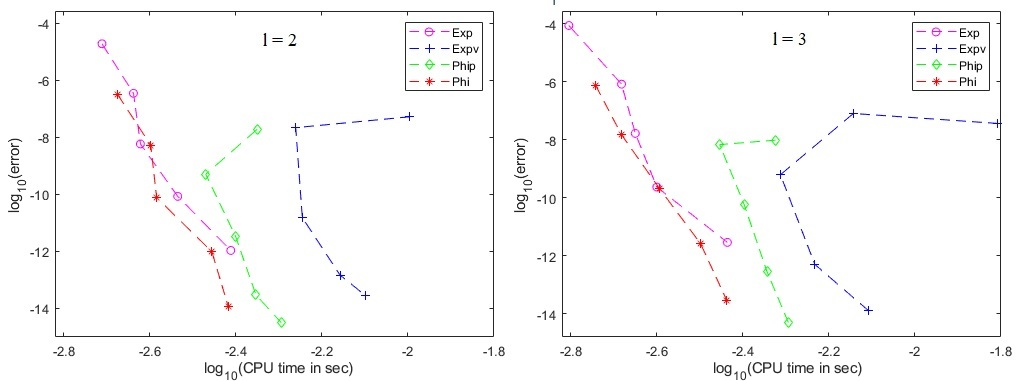
\includegraphics[scale=0.55]{Graphics/phil2l3.jpg}
	\caption{Diagrama tiempo-precisión para los métodos de \cite{hochbruck1997krylov}, \cite{sidje1998expokit}, \cite{niesen2012algorithm} y en (\ref{phi_approx}), denotados por \textit{Exp}, \textit{Expv}, \textit{Phip} y \textit{Phi} respectivamente, como función de la dimensión de Krylov $\mf$, en el cálculo de  (\ref{sum2_phiXv}) para dos valores de $l$. Izquierda $l=2$, Derecha $l=3$. De arriba hacia debajo, $\mf=4,5,6,7,8$ para cada método, siendo $\mf=6$ el valor óptimo estimado como se especificó anteriormente con tolerancias $ATol=10^{-9}$ y $RTol=10^{-6}$.}
	\label{fig:SumPhi}
\end{figure}

\subsubsection{Simulaciones numéricas con la aproximación Krylov-Padé libre de Jacobiano}
Consideraremos el cálculo de la combinación lineal (\ref{sum2_phiXv}) con matriz Jacobiana $f_x$ y campo vectorial $f$ del PVI resultante de discretizar una ecuación diferencial parcial. La siguiente matriz Jacobiana y la ecuación discretizada \redmark{fueron tomadas} de~\cite{tokman2006efficient}. 


	 Sean $u$ y $v$ vectores columna $N$-dimensionales. Con $x=[u^{\intercal}, v^{\intercal}]^{\intercal}$, se define la matriz Jacobiana de dimnesión $2N\times2N$
	\begin{equation} \label{ej:ej1-hpfj}
	f_{x}(x)=\left[ 
	\begin{array}{cc}
	diag(2u\cdot v-4) & diag(u\cdot u) \\ 
	diag(3-2u\cdot v) & -diag(u\cdot u)%
	\end{array}%
	\right] +\frac{\alpha }{(\Delta z)^{2}}\left[ 
	\begin{array}{cc}
	K & 0 \\ 
	0 & K%
	\end{array}%
	\right] ,
	\end{equation}
	\[
	K=\left[ 
	\begin{array}{ccccc}
	-2 & 1 &  &  & \\
	1 & -2 & 1 &  &  \\
	& \ddots  & \ddots  & \ddots  &  \\
	&  & 1 & -2 & 1 \\
	&  &  & 1 & -2%
	\end{array}%
	\right]_{N\times N} \, ,
	\]
	correspondiente al campo vectorial del sistema de $2N$ ecuaciones diferenciales ordinarias
	\begin{eqnarray*}
		\frac{du_{i}}{dt} &=&1+u_{i}^{2}v_{i}-4u_{i}+\frac{\alpha }{(\Delta z)^{2}}%
		(u_{i-1}-2u_{i}+u_{i+1}) \\
		\frac{dv_{i}}{dt} &=&3u_{i}-u_{i}^{2}v_{i}+\frac{\alpha }{(\Delta z)^{2}}%
		(v_{i-1}-2v_{i}+v_{i+1})
	\end{eqnarray*}
	que resulta de discretizar espacialmente las 2 ecuaciones en derivadas parciales conocidas como Brusselator 2D (ecuaciones del Ejemplo \ref{ex:Brus2D} en Capitulo \ref{chapter:lldp}), con $\alpha =1/50$, $u_{i}(0)=1+\sin (2\pi z_{i})$, $v_{i}(0)=3$, $z_{i}=i/(N+1)$, $\Delta z =1/(N+1)$, $i=1,\ldots,N$, y $N=800$. En la expresión para $f_x(x)$, $diag(.)$ es la operación de construir una matriz diagonal a partir de un vector y	
	\[  u \cdot v = [ u_1v_1, \ldots, u_Nv_N]^{\intercal}\, . \]
\importantcodes{JF1-Phi: método de Krylov-Padé libre de Jacobiano para aproximar  $t\varphi(tA)b$ con diferencias finitas de primer orden}
\importantcodes{JF2-Phi: método de Krylov-Padé libre de Jacobiano para aproximar  $t\varphi(tA)b$ con diferencias finitas de segundo orden}
Los códigos de Matlab \textit{JF1-Phi} y \textit{JF2-Phi} implementan la aproximación Krylov-Padé libre de Jacobiano de (\ref{phi_approx_fj}) con $\beta=0$ y las diferencias finitas de primer y segundo orden respectivamente
\begin{equation}\label{finite-differences}
	g(x,b;\delta)=\frac{f(x+\delta b)-f(x)}{\delta}  \;\;\; \text{y} \;\;\; g(x,b;\delta)=\frac{f(x+\delta b)-f(x-\delta b)}{2\delta}
\end{equation}
donde $\delta= \frac{\sqrt{(1+||x||_2)\epsilon_{mach}}}{\epsilon_{mach}+||b||_2}$ como se sugiere en~\cite{knoll2004jacobian}, siendo $\epsilon_{mach}$ el épsilon de la máquina. El código de Matlab \textit{Phi} implementa la aproximación Krylov-Padé en (\ref{phi_approx}) con la matriz exacta.

Utilizando la matrix Jacobiana (\ref{ej:ej1-hpfj}), la matriz y los vectores que definen a $M$ en (\ref{sum2_phiXv}) con $l=4$ se fijan como $A=f_x(x(0))$, $a_1=a_2=f(x(0))$, $a_3=2a_1 $ y $a_4=6a_1$. Con fines comparativos, el valor ``exacto'' de $e^{h M}$ en (\ref{sum2_phiXv}) y de $\me{\tau\overline{H}}$ en los códigos \textit{JF1-Phi}, \textit{JF2-Phi} y \textit{Phi} se calculan con la misma función de Matlab \textit{expm}. En los tres códigos, el valor de la dimensión de Krylov $\mf$ es determinado automáticamente dependiendo las tolerancias especificadas $Rtol$ y $Atol$, tal y como se explicó anteriormente. La norma euclidiana se utiliza para medir el error entre el valor ``exacto'' de $\lmatrix e^{h M}\rvector$ y sus aproximaciones.

La fila superior de la Figura \ref{fig:SumPhiBrusselator} presenta las gráficas $log$-$log$ de tolerancia relativa (\textit{Rtol}) contra error (\textit{error}) en el cálculo de (\ref{sum2_phiXv}) mediante las aproximaciones \textit{JF1-Phi}, \textit{JF2-Phi} y \textit{Phi} con tolerancias relativas y absolutas $Rtol=10^{-j}$ y $Atol=0$.$1 Rtol$, para $j=1,\ldots,6$. La fila inferior de esta figura presenta las gráficas de la dimensión de Krylov $\mf$ contra $log(Rtol)$ correspondientes a las aproximaciones en la fila superior de la figura.

\begin{figure}[htb]
	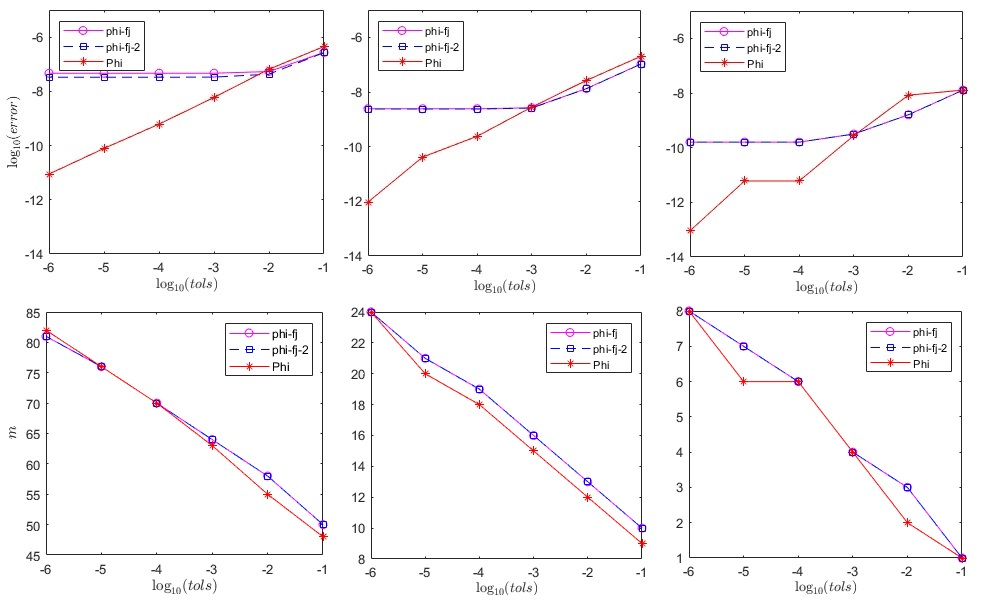
\includegraphics[scale=0.57]{Graphics/kpfj-brusselator-em.jpg}
	\caption{Superior: Gráficos $log-log$ de tolerancia relativa (\textit{rtol}) contra error (\textit{error}) en el cálculo de $\phi _{1}(f_x,h)a_{1}+\phi _{2}(f_x,h)a_{3}+\phi _{3}(f_x,h)a_{3}+\phi _{4}(f_x,h)a_{4}$ con la matriz Jacobiana $f_x$ (\ref{ej:ej1-hpfj}) mediante las aproximaciones \textit{JF1-Phi}, \textit{JF2-Phi} y \textit{Phi} con $rtol=10^{-j}$ y $j=1,\ldots,6$. De izquierda a derecha, con $h$=0.01,0.001,0.0001. Inferior: Gráficos de $log(rtol)$ contra dimensión de Krylov $\mf$ correspondiente a las aproximaciones de los gráfico superiores.}
	\label{fig:SumPhiBrusselator}
\end{figure}

Observe que una diferencia importante entre las aproximaciones libre de Jacobiano y las de matriz exacta es el umbral para los errores de las primeras a medida que disminuye la tolerancia. Como es de esperar, cuando la tolerancia $Rtol$ disminuye, la dimensión de Krylov $\mf$ para las tres aproximaciones aumenta y, en consecuencia, sus errores también disminuyen. Sin embargo, para valores crecientes de $\mf$, el valor fijo del segundo término de la derecha en (\ref{phi_approx_fj}) domina los valores decrecientes del primer término, lo que explica los umbrales para los errores de las aproximaciones libres de Jacobiano \textit{JF1-Phi} y \textit{JF2-Phi} en la Figura \ref{fig:SumPhiBrusselator}. Como se predice en (\ref{phi_approx}), el error de la aproximación con Jacobiano exacto \textit{Phi} en esta figura siempre disminuye cuando $\mf$ aumenta. Nótese también que, en correspondencia con el segundo término de la cota (\ref{phi_approx_fj}), la precisión de la aproximación con diferencia finita de segundo orden \textit{JF2-Phi} es ligeramente superior a la de la aproximación con diferencia finita de primer orden \textit{JF1-Phi} solo para los valores grandes de $h$ (gráfico superior izquierdo en la figura).

Las simulaciones numéricas corroboraron las principales implicaciones del análisis de error para la aproximación libre de Jacobiano, es decir, la existencia de un umbral para los errores cuando aumenta la dimensión del subespacio de Krylov, el menor error de la aproximación con diferencia finita de segundo orden y la menor precisión con respecto a la aproximacion que evalúa a la matriz Jacobiana exacta.

\subsubsection{Conclusiones del Capítulo}
En este Capítulo se construyeron aproximaciones Krylov-Padé con y sin la evaluación de Jacobiano para la solución de ecuaciones diferenciales lineales de dimensiones no pequeñas y se acotaron sus errores. Para cada aproximación, se propusieron novedosas estrategias para la estimación práctica de la dimensión de espacio Krylov, el orden de Padé y el error de aproximación. Se comprobó la eficacia de ambas aproximaciones para calcular la acción de funciones phi sobre vectores y, en ese aspecto, se
mostró las ventajas del uso de la aproximación Krylov-Padé con evaluación de Jacobiano en relación con otras aproximaciones similares existentes.

%Con el objetivo de solucionar de ecuaciones diferenciales lineales de dimensiones no pequeñas se construyeron las aproximaciones Krylov-Padé con y sin la evaluación de Jacobiano. Para ello se construye un subespacio de Krylov, se toman los dos primeros términos de la expansión en serie de $\varphi$ en dicho subespacio y luego es utilizada la aproximación de Padé para aproximar una exponencial de pequeñas dimensiones en este subespacio. Es importante notar que la aproximación Krylov-Padé sin la evaluación de Jacobiano es un extensión de la aproximación Krylov-Padé donde sustituyen los productos del Jacobiano por vector por alguna aproximación, mayormente se utiliza diferencias finitas.
%
%Además, para ambas aproximaciones se obtuvieron cotas teóricas de los errores de aproximación. Dichas cotas dependen de la dimensión del subespacio de Krylov, de los órdenes de Padé y, en el caso de la aproximación libre de Jacobiano, del orden utilizado para aproximar los productos del Jacobiano por vector. Otro aspecto importante es que se propusieron estrategias efectivas para la estimación práctica de la dimensión de espacio Krylov, el orden de Padé y el error de aproximación. A diferencia de otros trabajos, donde la dimensión del subespacio de Krylov se selecciona de un conjunto de dimensiones prefijad, la estrategia propuesta permite estimar la dimensión de Krylov óptima, en el sentido de que es la menor dimensión que satisface cierto error deseado.
%También se realizaron un conjunto de simulaciones numéricas donde se comprobó la eficacia de ambas aproximaciones para calcular la acción de funciones phi sobre vectores y, en ese aspecto, se mostró las ventajas del uso de la aproximación Krylov-Padé con evaluación de Jacobiano en relación con otras aproximaciones similares existentes
